\documentclass[../../main.tex]{subfiles}
\graphicspath{{\subfix{../../image/}}} % 指定图片目录,后续可以直接使用图片文件名。

% 例如:
% \begin{figure}[H]
% \centering
% \includegraphics[scale=0.4]{图.png}
% \caption{}
% \label{figure:图}
% \end{figure}
% 注意:上述\label{}一定要放在\caption{}之后,否则引用图片序号会只会显示??.

\begin{document}

\section{可测集与测度}

\begin{definition}[可测集]
设 \(E \subset \mathbb{R}^n\). 若对任意的点集 \(T \subset \mathbb{R}^n\), 有
\begin{align*}
m^*(T)=m^*(T \cap E)+m^*(T \cap E^c), 
\end{align*}
则称 \(E\) 为 \textbf{Lebesgue 可测集}(或 \textbf{\(m^*\)-可测集})或$E$\textbf{可测}, 简称为\textbf{可测集}, 其中 \(T\) 称为\textbf{试验集}(这一定义可测集的等式也称为 \textbf{Carathéodory条件}). 可测集的全体称为\textbf{可测集类}, 简记为 \(\mathscr{M}\). 
\end{definition}

\begin{theorem}[集合可测的充要条件]\label{theorem:可测的充要条件}
设\(E\subset \mathbb{R}^n\), 则$E\in \mathscr{M}$的充要条件是对任一点集 \(T \subset \mathbb{R}^n\)且\(m^*(T)< + \infty\),都有
\begin{align}
m^*(T) \geqslant  m^*(T \cap E)+m^*(T \cap E^c) \label{eq:2.3}
\end{align}
成立. 
\end{theorem}
\begin{remark}
往后经常利用这个定理的充分性来证明一个集合可测.但这个定理的必要性要弱于可测集的定义.
\end{remark}
\begin{proof}
必要性由可测集的定义立得.下证充分性.
由外测度的次可加性可得
\[
m^*(T)=m^*\left( T\cap \mathbb{R} ^n \right) =m^*\left( T\cap \left( E\cup E^c \right) \right) =m^*\left( \left( T\cap E \right) \cup \left( T\cap E^c \right) \right)  \leqslant  m^*(T \cap E)+m^*(T \cap E^c)
\]
总是成立的. 又因为在 \(m^*(T)=\infty\) 时 \eqref{eq:2.3} 式总成立,故对任意的点集 \(T \subset \mathbb{R}^n\),都有
\begin{align*}
m^*(T)=m^*(T \cap E)+m^*(T \cap E^c), 
\end{align*}
即$E\in \mathscr{M}$.

\end{proof}

\begin{definition}[零测集]
外测度为零的点集称为\textbf{零测集}. 
\end{definition}
\begin{remark}
显然, \(\mathbb{R}^n\) 中由单个点组成的点集是零测集. 从而根据外测度的次可加性知道 \(\mathbb{R}^n\) 中的有理点集 \(\mathbb{Q}^n\) 是零测集.
\end{remark}

\begin{proposition}\label{proposition:零测集的基本性质}
\begin{enumerate}
\item 零测集的任一子集是零测集.

\item 零测集一定可测,即若 \(m^*(E)=0\), 则 \(E \in \mathscr{M}\). 
\end{enumerate}
\end{proposition}
\begin{proof}
\begin{enumerate}
\item 由外测度的单调性立得.

\item 事实上, 此时我们有
\begin{align*}
m^*(T \cap E)+m^*(T \cap E^c) \leqslant  m^*(E)+m^*(T)=m^*(T).
\end{align*}
再由\refthe{theorem:可测的充要条件}立得.
\end{enumerate}

\end{proof}

\begin{proposition}\label{proposition:外测度的可加性的条件}
若 \(E_1 \subset S\), \(E_2 \subset S^c\), \(S \in \mathscr{M}\), 则有
\begin{align*}
m^*(E_1 \cup E_2) = m^*(E_1) + m^*(E_2).
\end{align*}
\end{proposition}
\begin{remark}
这个命题表明:当两个集合由一个可测集分离开时, 其外测度就有可加性.
\end{remark}
\begin{proof}
事实上, 此时取试验集 \(T = E_1 \cup E_2\), 从 \(S\) 是可测集的定义得
\begin{align*}
m^*(E_1 \cup E_2) = m^*((E_1 \cup E_2) \cap S) + m^*((E_1 \cup E_2) \cap S^c) = m^*(E_1) + m^*(E_2).
\end{align*}

\end{proof}

\begin{corollary}\label{corollary:2个无交可测集与任意集合的并的外测度的性质}
当 \(E_1\) 与 \(E_2\) 是互不相交的可测集时, 对任一集合 \(T\) 有
\begin{align*}
m^*(T \cap (E_1 \cup E_2)) =m^*((T\cap E_1)\cup (T\cap E_2))= m^*(T \cap E_1) + m^*(T \cap E_2).
\end{align*} 
\end{corollary}
\begin{proof}
注意到$T\cap E_1\in E_1$,$T\cap E_2\in E_1^c$,而$E_1\in \mathscr{M}$,故由集合运算的性质和\refpro{proposition:外测度的可加性的条件}可知
\begin{align*}
m^*(T \cap (E_1 \cup E_2))=m^*((T\cap E_1)\cup (T\cap E_2)) = m^*(T \cap E_1) + m^*(T \cap E_2).
\end{align*} 

\end{proof}

\begin{corollary}\label{corollary:有限个无交可测集与任意集合的并的外测度的性质}
当$E_1,E_2,\cdots,E_n$是互不相交的可测集时,对任一集合$T$有
\begin{align*}
m^*\left(T\cap\bigcup_{k=1}^nE_k\right) = m^*\left(\bigcup_{k=1}^n\left(T\cap E_k\right)\right) = \sum_{k=1}^n m^*(T\cap E_k).
\end{align*}
\end{corollary}
\begin{proof}
当$n=1$时, 结论显然成立.假设当$n=m$时结论成立,考虑$n=m+1$的情况.由于$E_1,E_2,\cdots,E_{m+1}$皆互不相交,因此$\bigcup_{k=1}^m{E_k}$和$E_{m+1}$也互不相交.于是由集合运算的性质和\refcor{corollary:2个无交可测集与任意集合的并的外测度的性质}以及归纳假设可得
\begin{align*}
&m^*\left( T\cap \bigcup_{k=1}^{m+1}{E_k} \right) =m^*\left( \bigcup_{k=1}^{m+1}{\left( T\cap E_k \right)} \right) =m^*\left( T\cap \left( \bigcup_{k=1}^m{E_k}\cup E_{m+1} \right) \right) =m^*\left( \left( T\cap \bigcup_{k=1}^m{E_k} \right) \cup \left( T\cap E_{m+1} \right) \right) 
\\
&=m^*\left( T\cap \bigcup_{k=1}^m{E_k} \right) +m^*\left( T\cap E_{m+1} \right) =\sum_{k=1}^m{m^*\left( T\cap E_k \right)}+m^*\left( T\cap E_{m+1} \right) =\sum_{k=1}^{m+1}{m^*\left( T\cap E_k \right)}.
\end{align*}
故由数学归纳法可知结论成立.

\end{proof}

\begin{theorem}[可测集的性质]\label{theorem:可测集的性质}
\begin{enumerate}[(1)]
\item \(\varnothing \in \mathscr{M}\).
\item 若 \(E \in \mathscr{M}\), 则 \(E^c \in \mathscr{M}\).

\item 若 \(E_1 \in \mathscr{M}\), \(E_2 \in \mathscr{M}\), 则 \(E_1 \cup E_2\), \(E_1 \cap E_2\) 以及 \(E_1 \setminus E_2\) 皆属于 \(\mathscr{M}\). (由此知, 可测集任何有限次取交、并运算后所得的集皆为可测集. )
\item 若 \(E_i \in \mathscr{M}\) (\(i = 1,2,\cdots\)), 则其并集$\bigcup_{i = 1}^{\infty} E_i$也属于 \(\mathscr{M}\). 若进一步有 \(E_i \cap E_j = \varnothing\) (\(i \neq j\)), 则
\begin{align*}
m^*\left(\bigcup_{i = 1}^{\infty} E_i\right) = \sum_{i = 1}^{\infty} m^*(E_i),
\end{align*}
即 \(m^*\) 在 \(\mathscr{M}\) 上满足\textbf{可数可加性}(或称为 \(\sigma -\)可加性).

\item 若 \(E_i \in \mathscr{M}\) (\(i = 1,2,\cdots\)), 则其交集$\bigcap_{i = 1}^{\infty} E_i$也属于 \(\mathscr{M}\). 

\item 如果$A$和$B$分别为$p$维和$q$维空间的可测集,那么$A\times B$是$p + q$维空间的可测集,测度为
\begin{align*}
m(A\times B)=m(A)\cdot m(B).
\end{align*}
\end{enumerate}
\end{theorem}
\begin{proof}
\begin{enumerate}[(1)]
\item 显然成立.
\item 注意到 \((E^c)^c = E\), 从定义可立即得出结论.
\item 对于任一集 \(T \subset \mathbb{R}^n\), 根据集合分解(参阅\hyperref[figure:集合关系示意图1]{图\ref{figure:集合关系示意图1}})与外测度的次可加性, 我们有
\begin{align*}
m^*(T) &\leqslant  m^*(T \cap (E_1 \cup E_2)) + m^*(T \cap (E_1 \cup E_2)^c) \\
&= m^*(T \cap (E_1 \cup E_2)) + m^*((T \cap E_1^c) \cap E_2^c) \\
&\leqslant  m^*((T \cap E_1) \cap E_2) + m^*((T \cap E_1) \cap E_2^c) \\
&\quad + m^*((T \cap E_1^c) \cap E_2) + m^*((T \cap E_1^c) \cap E_2^c).
\end{align*}
又由 \(E_1\), \(E_2\) 的可测性知, 上式右端就是
\begin{align*}
m^*(T \cap E_1) + m^*(T \cap E_1^c) = m^*(T).
\end{align*}
这说明
\begin{align*}
m^*(T) = m^*(T \cap (E_1 \cup E_2)) + m^*(T \cap (E_1 \cup E_2)^c).
\end{align*}
也就是说 \(E_1 \cup E_2\) 是可测集.
\begin{figure}[H]
\centering
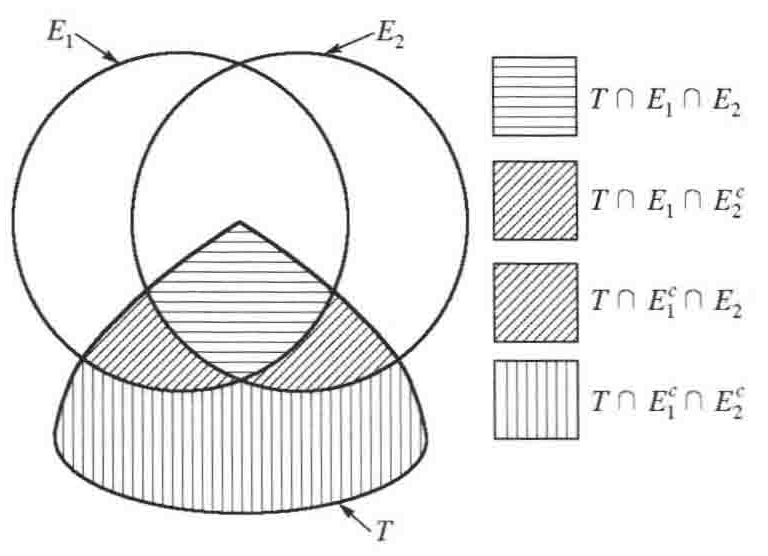
\includegraphics[scale=0.3]{集合关系示意图1}
\caption{}
\label{figure:集合关系示意图1}
\end{figure}
为证 \(E_1 \cap E_2\) 是可测集, 只需注意 \(E_1 \cap E_2 = (E_1^c \cup E_2^c)^c\) 即可. 又由 \(E_1 \setminus E_2 = E_1 \cap E_2^c\) 可知, \(E_1 \setminus E_2\) 是可测集. 
\item 首先, 设 \(E_1\), \(E_2\), \(\cdots\), \(E_i\), \(\cdots\) 皆互不相交, 并令
\[
S = \bigcup_{i = 1}^{\infty} E_i, \quad S_k = \bigcup_{i = 1}^k E_i, \quad k = 1,2,\cdots.
\]
由(3)知每个 \(S_k\) 都是可测集, 从而对任一集 \(T\), 我们有
\begin{align*}
m^*(T) &= m^*(T \cap S_k) + m^*(T \cap S_k^c) \\
&= m^*\left(\bigcup_{i = 1}^k (T \cap E_i)\right) + m^*(T \cap S_k^c) \\
&\xlongequal{\text{\refcor{corollary:有限个无交可测集与任意集合的并的外测度的性质}}} \sum_{i = 1}^k m^*(T \cap E_i) + m^*(T \cap S_k^c).
\end{align*}
由于 \(T \cap S_k^c \supset T \cap S^c\), 可知
\begin{align*}
m^*(T) \geqslant  \sum_{i = 1}^k m^*(T \cap E_i) + m^*(T \cap S^c).
\end{align*}
令 \(k \to \infty\), 就有
\begin{align*}
m^*(T) \geqslant  \sum_{i = 1}^{\infty} m^*(T \cap E_i) + m^*(T \cap S^c).
\end{align*}
再由外测度的次可加性可得
\begin{align*}
m^*(T)&\geqslant \sum_{i=1}^{\infty}{m^*(T}\cap E_i)+m^*(T\cap S^c)\geqslant m^*(\bigcup_{i=1}^{\infty}{\left( T\cap E_i \right)})+m^*(T\cap S^c)
\\
&=m^*(T\cap \bigcup_{i=1}^{\infty}{E_i})+m^*(T\cap S^c)=m^*(T\cap S)+m^*(T\cap S^c).
\end{align*}
这说明 \(S \in \mathscr{M}\).
此外, 在公式
\begin{align*}
m^*(T) \geqslant  \sum_{i = 1}^{\infty} m^*(T \cap E_i) + m^*(T \cap S^c)
\end{align*}
中以 \(T \cap S\) 替换 \(T\), 则又可得
\begin{align*}
m^*(T \cap S) \geqslant  \sum_{i = 1}^{\infty} m^*(T \cap E_i).
\end{align*}
又由外测度的次可加性可知反向不等式总是成立的, 因而实际上有
\begin{align*}
m^*(T \cap S) = \sum_{i = 1}^{\infty} m^*(T \cap E_i).
\end{align*}
在这里再取 \(T\) 为全空间 \(\mathbb{R}^n\), 就可证明可数可加性质:
\begin{align*}
m^*(S) = m^*\left(\bigcup_{i = 1}^{\infty} E_i\right) = \sum_{i = 1}^{\infty} m^*(E_i).
\end{align*}

其次, 对于一般的可测集列 \(\{E_i\}\), 我们令
\[
S_1 = E_1, \quad S_k = E_k \setminus \left(\bigcup_{i = 1}^{k - 1} E_i\right), \quad k \geqslant  2,
\]
则 \(\{S_k\}\) 是互不相交的可测集列. 而由 \(\bigcup_{i = 1}^{\infty} E_i = \bigcup_{k = 1}^{\infty} S_k\) 可知, \(\bigcup_{i = 1}^{\infty} E_i\) 是可测集.

\item 由(2)可知$E_i^c\in \mathscr{M}$,再由(4)可知$\bigcup_{i = 1}^{\infty} E_i^c$.于是再利用(2)和De Morgan定律可得
\begin{align*}
\left( \bigcup_{i=1}^{\infty}{E_{i}^{c}} \right) ^c=\bigcap_{i=1}^{\infty}{E_i}\in \mathscr{M} .
\end{align*}

\item 证明见\href{https://zhuanlan.zhihu.com/p/365546947#:~:text=%E5%AE%9A%E7%90%864.1%20%EF%BC%88%E5%8F%AF%E6%B5%8B%E9%9B%86%E7%9A%84%E7%9B%B4%E7%A7%AF%E4%BB%8D%E7%84%B6%E5%8F%AF%E6%B5%8B%EF%BC%8C%E5%B9%B6%E4%B8%94%E7%9B%B4%E7%A7%AF%E7%9A%84%E6%B5%8B%E5%BA%A6%E4%B8%BA%E6%B5%8B%E5%BA%A6%E7%9A%84%E4%B9%98%E7%A7%AF%EF%BC%89%20%E5%A6%82%E6%9E%9C%20A%20%E5%92%8C%20B%20%E5%88%86%E5%88%AB%E4%B8%BA%20p,%28A%29%20cdot%20m%20%28B%29%5C%20%E8%AF%81%E6%98%8E%E6%8C%89%E7%85%A7%E4%BB%A5%E4%B8%8B%E7%89%B9%E6%AE%8A%E5%88%B0%E4%B8%80%E8%88%AC%E7%9A%84%E8%BF%87%E7%A8%8B%E3%80%82%20%E6%96%B9%E4%BD%93%EF%BC%9A%E6%96%B9%E4%BD%93%E7%9A%84%E7%9B%B4%E7%A7%AF%E4%BB%8D%E7%84%B6%E6%98%AF%E6%96%B9%E4%BD%93%EF%BC%8C%E6%89%80%E4%BB%A5%E5%8F%AF%E6%B5%8B%E3%80%82%20%E5%85%B6%E6%B5%8B%E5%BA%A6%E5%B0%B1%E6%98%AF%E5%8E%9F%E6%9D%A5%E4%B8%A4%E4%B8%AA%E6%96%B9%E4%BD%93%E7%9A%84%E4%B9%98%E7%A7%AF%E3%80%82%20%E6%A0%B9%E6%8D%AE%E6%B5%8B%E5%BA%A6%E7%9A%84%E5%8F%AF%E5%8A%A0%E6%80%A7%E5%BE%97%E5%88%B0%E7%9B%B4%E7%A7%AF%E7%9A%84%E6%B5%8B%E5%BA%A6%E7%AD%89%E4%BA%8E%E6%B5%8B%E5%BA%A6%E7%9A%84%E4%B9%98%E7%A7%AF%E3%80%82}{知乎专栏}.
\end{enumerate} 

\end{proof}

\begin{corollary}\label{corollary:可测集类是sigma-代数}
$\mathscr{M}$是$\mathbb{R}^n$上的一个$\sigma$-代数.
\end{corollary}
\begin{proof}
由\hyperref[theorem:可测集的性质]{可测集的性质(1)(2)(4)}立得.

\end{proof}


\begin{proposition}\label{proposition:Cantor集可测且测度为0}
证明:Cantor集C是可测的,并且$m(C)=0$.
\end{proposition}
\begin{proof}
开区间是可测的. 由\hyperref[theorem:开集构造定理]{开集构造定理}, 我们知道 \(\mathbb{R}\) 中的开集是开区间的可数并, 因此也可测. 因此, 闭集也是可测的. 显然, 每个 \(C_n\) 都是闭集. 并且
\begin{align*}
C = \bigcap_{n = 1}^{\infty} C_n
\end{align*}
于是 \(C\) 也是闭集. 因此 \(C\) 是可测的.

下面, 我们用两种方法计算康托集的测度.

{\color{blue}法一:}根据我们的构造, \(C_{n + 1}\) 的测度刚好是去掉了 \(1/3\) 的 \(C_n\) 的测度. 换言之,
\begin{align*}
m(C_{n + 1}) = \left(1 - \frac{1}{3}\right)m(C_n) = \frac{2}{3}m(C_n)
\end{align*}
递归地, 对任意 \(n \in \mathbb{N}\), 我们有
\begin{align*}
m(C_n) = \left(\frac{2}{3}\right)^n m(C_0) = \left(\frac{2}{3}\right)^n
\end{align*}
注意到
\begin{align*}
m(C_0) = 1 < \infty
\end{align*}
因此由测度的第二单调收敛定理,
\begin{align*}
m(C) = m\left(\bigcap_{n = 1}^{\infty} C_n\right) = \lim_{n \to \infty} m(C_n) = \lim_{n \to \infty} \left(\frac{2}{3}\right)^n = 0
\end{align*}
此即得证.

{\color{blue}法二:}设 \(n \geqslant  2\). \(C_n\) 比 \(C_{n - 1}\) 减少了 \(2^{n - 1}\) 个区间, 每个区间长度为 \(\frac{1}{3^n}\). 因此 \(C_n\) 比 \(C_{n - 1}\) 减少的长度为
\begin{align*}
2^{n - 1}\frac{1}{3^n} = \frac{1}{3}\left(\frac{2}{3}\right)^{n - 1}
\end{align*}
总共减少的长度为
\begin{align*}
\sum_{n = 1}^{\infty} \frac{1}{3}\left(\frac{2}{3}\right)^{n - 1} = \frac{1}{3} \frac{1}{1 - \frac{2}{3}} = \frac{1}{3} \cdot 3 = 1
\end{align*}
因此
\begin{align*}
m(C) = 1 - 1 = 0.
\end{align*} 

\end{proof}

\begin{proposition}\label{proposition:可测集类的基数是2^c}
\(\mathscr{M}\) 的基数是 \(2^c\).
\end{proposition}
\begin{proof}
由\refpro{proposition:Cantor集可测且测度为0}可知Cantor集是零测集,不难推断 \(\mathscr{M}\) 的基数大于或等于 \(2^c\), 但 \(\mathscr{M}\) 的基数又不会超过 \(2^c\), 于是 \(\mathscr{M}\) 的基数实际上是 \(2^c\). 

\end{proof}

\begin{definition}[Lebesgue测度]
对于可测集 \(E\), 其外测度称为\textbf{测度}, 记为 \(m(E)\). 这就是通常所说的 \(\mathbb{R}^n\) 上的 \textbf{Lebesgue测度}.
\end{definition}

\begin{definition}[测度]
设 \(X\) 是非空集合, \(\mathscr{A}\) 是 \(X\) 的一些子集构成的 \(\sigma -\)代数. 若 \(\mu\) 是定义在 \(\mathscr{A}\) 上的一个集合函数, 且满足:
\begin{enumerate}[(i)]
\item \(0 \leqslant  \mu(E) \leqslant  +\infty\) (\(E \in \mathscr{A}\));
\item \(\mu(\varnothing)=0\);
\item \(\mu\) 在 \(\mathscr{A}\) 上是可数可加的,
\end{enumerate}
则称 \(\mu\) 是 \(\mathscr{A}\) 上的(非负)\textbf{测度}. \(\mathscr{A}\) 中的元素称为(\(\mu\))\textbf{可测集}, 有序组 \((X, \mathscr{A}, \mu)\) 称为\textbf{测度空间}. 
\end{definition}
\begin{remark}
由\refcor{corollary:可测集类是sigma-代数}可知$\mathscr{M}$就是$\mathbb{R}^n$上的一个$\sigma$-代数,故本节所建立的测度空间就是 \((\mathbb{R}^n, \mathscr{M}, m)\). 
\end{remark}

\begin{theorem}[测度的基本性质]\label{theorem:测度的基本性质}
\begin{enumerate}[(1)]
\item 非负性: 若$E\in \mathscr{M}$,则\(m(E) \geqslant  0\), \(m(\varnothing)=0\);

\item 单调性: 若$E_1,E_2\in \mathscr{M}$且\(E_1 \subset E_2\), 则 \(m(E_1) \leqslant  m(E_2)\).

并且若还有$m(E_1)<+\infty$,则$m(E_2\setminus E_1)=m(E_1)-m(E_2)$.

\item 可数可加性: 若 \(E_i \in \mathscr{M}\) (\(i = 1,2,\cdots\))且 \(E_i \cap E_j = \varnothing\) (\(i \neq j\)),则
\begin{align*}
m\left(\bigcup_{i = 1}^{\infty} E_i\right) = \sum_{i = 1}^{\infty} m(E_i).
\end{align*}

\item 若$E_1,E_2\in \mathscr{M}$,且$m(E_1\cap E_2)<+\infty$,则$m(E_1\cup E_2)=m(E_1)+m(E_2)-m(E_1\cap E_2)$.
\end{enumerate}
\end{theorem}
\begin{proof}
\begin{enumerate}[(1)]
\item 由\hyperref[theorem:R^n 中点集的外测度性质]{$R^n$ 中点集的外测度性质}立得.

\item 由\hyperref[theorem:R^n 中点集的外测度性质]{$R^n$ 中点集的外测度性质}可知\(m(E_1) \leqslant  m(E_2)\).再根据$E_1$可测的定义可知
\begin{align*}
m^*\left( E_2 \right) =m^*\left( E_2\cap E_1 \right) +m^*\left( E_2\cap E_{1}^{c} \right) =m^*\left( E_1 \right) +m^*\left( E_2\setminus E_1 \right) .
\end{align*}
又由\hyperref[theorem:可测集的性质]{可测集的性质}可知$E_2\setminus E_1$可测,又因为$E_1,E_2$可测,所以上式等价于
\begin{align*}
m\left( E_2 \right) =m\left( E_2\cap E_1 \right) +m\left( E_2\cap E_{1}^{c} \right) =m\left( E_1 \right) +m\left( E_2\setminus E_1 \right) .
\end{align*}
又$m(E_1)<+\infty$,故由上式移项后得$m(E_2\backslash E_1)=m(E_2)-m(E_1).$

\item 由\hyperref[theorem:可测集的性质]{可测集的性质}立得.

\item 注意到$E_1\cap (E_2\backslash (E_1\cap E_2))=\varnothing$,并且$E_1\cap E_2\subset E_2,m(E_1\cap E_2)<+\infty$,故由(2)(3)可得
\begin{align*}
m\left( E_1\cup E_2 \right) =m\left[ E_1\cup \left( E_2\backslash (E_1\cap E_2) \right) \right] =m\left( E_1 \right) +m\left[ E_2\backslash (E_1\cap E_2) \right] =m\left( E_1 \right) +m\left( E_2 \right) -m\left( E_1\cap E_2 \right) .
\end{align*}
\end{enumerate}

\end{proof}

\begin{theorem}[递增可测集列的测度运算]\label{theorem:递增可测集列的测度运算}
若有递增可测集列$E_1\subset E_2\subset\cdots\subset E_k\cdots$,则
\begin{align}
m\left(\lim_{k\to\infty}E_k\right)=\lim_{k\to\infty}m(E_k).\label{eq:2.4}
\end{align}
\end{theorem}
\begin{proof}
若存在$k_0$,使得$m(E_{k_0})=+\infty$,则
\begin{align*}
m^*\left(\lim_{k\rightarrow \infty}E_k\right) = m^*\left(\bigcup_{k=1}^{\infty}E_k\right)\geqslant m^*(E_{k_0}).
\end{align*}
因此$m^*\left(\lim_{k\rightarrow \infty}E_k\right) = +\infty$. 又由$\{E_k\}_{k=1}^{\infty}$递增可知
\begin{align*}
m^*(E_k) \geqslant m^*(E_{k_0}), \quad \forall k \geqslant k_0.
\end{align*}
因此$\lim_{k\rightarrow \infty}m^*(E_k) = +\infty$.
故此时定理自然成立。

现在假定对一切$k$,有$m(E_k)<+\infty$。由假设$E_k\in\mathscr{M}$($k = 1,2,\cdots$),故$E_{k - 1}$与$E_k\setminus E_{k - 1}$是互不相交的可测集。由测度的可加性知
$m(E_{k - 1})+m(E_k\setminus E_{k - 1})=m(E_k)$。
因为$m(E_{k - 1})$是有限的,所以移项得
$m(E_k\setminus E_{k - 1})=m(E_k)-m(E_{k - 1})$。
令$E_0 = \varnothing$,可得
$\lim_{k\to\infty}E_k=\bigcup_{k = 1}^{\infty}E_k=\bigcup_{k = 1}^{\infty}(E_k\setminus E_{k - 1})$。
再应用\hyperref[theorem:测度的基本性质]{测度的可数可加性},我们有
\begin{align*}
m\left(\lim_{k\to\infty}E_k\right)&=m\left(\bigcup_{k = 1}^{\infty}(E_k\setminus E_{k - 1})\right)
=\sum_{k = 1}^{\infty}(m(E_k)-m(E_{k - 1}))\\
&=\lim_{k\to\infty}\sum_{i = 1}^{k}(m(E_i)-m(E_{i - 1}))
=\lim_{k\to\infty}m(E_k).
\end{align*}

\end{proof}

\begin{corollary}[递减可测集列的测度运算]\label{corollary:递减可测集列的测度运算}
若有递减可测集列$E_1\supset E_2\supset\cdots\supset E_k\supset\cdots$,且$m(E_1)<+\infty$,则
\begin{align}
m\left(\lim_{k\to\infty}E_k\right)=\lim_{k\to\infty}m(E_k).\label{eq:2.5}
\end{align}
\end{corollary}
\begin{proof}
由\hyperref[theorem:可测集的性质]{可测集的性质(5)}可知$\lim_{k\to\infty}E_k$是可测集,再由\hyperref[theorem:测度的基本性质]{测度的单调性}可知$\lim_{k\to\infty}m(E_k)\leqslant  m(E_1)<+\infty$.因为
$E_1\setminus E_k\subset E_1\setminus E_{k + 1},k = 2,3,\cdots$,
所以由\hyperref[theorem:可测集的性质]{可测集的性质(2)}可知$\{E_1\setminus E_k\}$是递增可测集合列。于是由\hyperref[theorem:递增可测集列的测度运算]{递增可测集列的测度运算}可知
\begin{align*}
m\left(E_1\setminus\lim_{k\to\infty}E_k\right)=m\left(\lim_{k\to\infty}(E_1\setminus E_k)\right)
=\lim_{k\to\infty}m(E_1\setminus E_k).
\end{align*}
由于$m(E_1)<+\infty$,故由\hyperref[theorem:测度的基本性质]{测度的基本性质(2)}上式可写为
$m(E_1)-m\left(\lim_{k\to\infty}E_k\right)=m(E_1)-\lim_{k\to\infty}m(E_k)$。
消去$m(E_1)$,我们有
$m\left(\lim_{k\to\infty}E_k\right)=\lim_{k\to\infty}m(E_k)$。 

\end{proof}

\begin{theorem}\label{theorem:可测集的Fatou引理}
\begin{enumerate}[(1)]
\item 若有可测集列$\{E_k\}$,且有$\sum_{k = 1}^{\infty}m(E_k)<+\infty$,则
\begin{align*}
m\left(\varlimsup_{k\to\infty}E_k\right)= 0.
\end{align*}

\item 设$\{E_k\}$是可测集列,则
\begin{align*}
m\left(\varliminf_{k\to\infty}E_k\right)\leqslant\varliminf_{k\to\infty}m(E_k),\quad m\left(\varlimsup_{k\to\infty}E_k\right)\geqslant\varlimsup_{k\to\infty}m(E_k).
\end{align*}
\end{enumerate}
\end{theorem}
\begin{remark}
也称结论
\begin{align*}
m\left(\varliminf_{n\to\infty}E_n\right)\leqslant\varliminf_{n\to\infty}m(E_n),\quad m\left(\varlimsup_{n\to\infty}E_n\right)\geqslant\varlimsup_{n\to\infty}m(E_n)
\end{align*}
为测度论中的 Fatou 引理(见第四章).
\end{remark}
\begin{proof}
\begin{enumerate}
\item \begin{align*}
m\left( \underset{k\rightarrow \infty}{\overline{\lim }}E_k \right) &=m\left( \bigcap_{k=1}^{\infty}{\bigcup_{i=k}^{\infty}{E_i}} \right) =m\left( \lim_{k\rightarrow \infty} \bigcup_{i=k}^{\infty}{E_i} \right) 
\\
&\xlongequal{\text{\hyperref[corollary:递减可测集列的测度运算]{递减可测集列的测度运算}}}\lim_{k\rightarrow \infty} m\left( \bigcup_{i=k}^{\infty}{E_i} \right) \\
&\leqslant \lim_{k\rightarrow \infty} \sum_{i=k}^{\infty}{m(E_i)}=0.
\end{align*}

\item 因为$\bigcap_{j = k}^{\infty}E_j\subset E_k,\bigcup_{i = k}^{\infty}E_i\supset E_k$($k = 1,2,\cdots$),所以有
\begin{align*}
m\left(\bigcap_{j = k}^{\infty}E_j\right)\leqslant m(E_k),\quad m\left(\bigcup_{i = k}^{\infty}E_i\right)\geqslant m(E_k)\quad (k = 1,2,\cdots).
\end{align*}
令$k\to\infty$,则得($\bigcap_{j = k}^{\infty}E_j$随$k$增大而递增,$\bigcup_{i = k}^{\infty}E_i$随$k$增大而递减)
\begin{align*}
m\left( \underset{k\rightarrow \infty}{\underline{\lim }}E_k \right) &=m\left( \bigcup_{k=1}^{\infty}{\bigcap_{j=k}^{\infty}{E_j}} \right) =m\left( \lim_{k\rightarrow \infty} \bigcap_{j=k}^{\infty}{E_j} \right) 
\\
&\xlongequal{\text{\hyperref[theorem:递增可测集列的测度运算]{递增可测集列的测度运算}}}\lim_{k\rightarrow \infty} m\left( \bigcap_{j=k}^{\infty}{E_j} \right) \\
&\leqslant \underset{k\rightarrow \infty}{\underline{\lim }}m(E_k).
\end{align*}
\begin{align*}
m\left( \underset{k\rightarrow \infty}{\overline{\lim }}E_k \right) &=m\left( \bigcap_{k=1}^{\infty}{\bigcup_{i=k}^{\infty}{E_i}} \right) =m\left( \lim_{k\rightarrow \infty} \bigcup_{i=k}^{\infty}{E_i} \right) 
\\
&\xlongequal{\text{\hyperref[corollary:递减可测集列的测度运算]{递减可测集列的测度运算}}}\lim_{k\rightarrow \infty} m\left( \bigcup_{i=k}^{\infty}{E_i} \right) \\
&\geqslant \underset{k\rightarrow \infty}{\overline{\lim }}m(E_k).
\end{align*}
\end{enumerate} 

\end{proof}

































\end{document}